%
%----------------------------------------------------------------------------------------
%	PACKAGES AND DOCUMENT CONFIGURATIONS
%----------------------------------------------------------------------------------------
%

\documentclass[12pt]{article} %report, article, amsart, exam
\usepackage[letterpaper,margin=1in]{geometry}
\usepackage{fancyhdr,color}
\usepackage{tikz,graphicx,multicol}
\usepackage{amssymb,euscript,eufrak,nicefrac,enumitem}
\usepackage{amsfonts,amsmath,amsthm} %don't need with 'amsart' document class
\usepackage{hyperref}
\usepackage{comment}
\usepackage{scrextend} %needed for addmargin environment
\usepackage{graphicx} 
\usepackage{listings}

\usepackage{color}
\usepackage{accsupp}
\usepackage{booktabs}
\usepackage{subcaption}

\definecolor{dkblue}{rgb}{0,0,0.5}
\definecolor{comment}{rgb}{1,0,0}
\definecolor{mauve}{rgb}{.627,.126,.941}
\definecolor{purple}{rgb}{0.5, 0, 0.545098}

\lstdefinestyle{customc}{
  belowcaptionskip=1\baselineskip,
  breaklines=true,
  frame=L,
  xleftmargin=\parindent,
  language=C,
  showstringspaces=false,
  basicstyle=\footnotesize\ttfamily,
  keywordstyle=\bfseries\color{green!40!black},
  commentstyle=\itshape\color{purple!40!black},
  identifierstyle=\color{blue},
  stringstyle=\color{orange},
}

\lstdefinestyle{customasm}{
  belowcaptionskip=1\baselineskip,
  frame=L,
  xleftmargin=\parindent,
  language=[x86masm]Assembler,
  basicstyle=\footnotesize\ttfamily,
  commentstyle=\itshape\color{purple!40!black},
}

\lstset{escapechar=@,style=customc}

%
%----------------------------------------------------------------------------------------
%% Define headers & footers
%----------------------------------------------------------------------------------------

\pagestyle{fancy}
   \lhead{} 
   %\chead{Loyola University Chicago} 
   \rhead{}
   \renewcommand{\headrulewidth}{0pt}
   \addtolength{\footnotesep}{5mm}
 
%
%----------------------------------------------------------------------------------------
%% Some user-defined colors
%----------------------------------------------------------------

\setlength{\parskip}{1em}
\renewcommand{\baselinestretch}{1.3}

%
%----------------------------------------------------------------------------------------
%% BEGIN: topmatter
%----------------------------------------------------------------------------------------
%

\title{ COMP 464 - High Performance Computing \\ OpenMP Threading} % Title
\author{
Loyola University Chicago \\
Jose Luis Rodriguez 
} % Author name
\date{\today} % Date for the report

%
%% END: topmatter
%%------------------------------

\begin{document}

\maketitle

\thispagestyle{fancy}

%---------------------------------------------------------------------------------------- 
%	SECTION 1 - PROBLEM STATEMENT
%----------------------------------------------------------------------------------------

\section{Overview}

This report highlights the procedures and results of running the nbody3 C++ code that predicts the individual motion of a group of celestial objects (particles) interacting with each other gravitationally. The program also runs a series of experiments and generates a benchmark (max, min and average speed) utilizing the Stampede2 supercomputer at The University of Texas at Austin?s Texas Advanced Computing Center (TACC). The nbody3 code utilize Intel C++ library compilers and the OpenMP library in order to parallelize the serial code details and speci?cations to follow.

The n-body problem code performs two major benchmarks in order to compute strong scalability and weak scalability. The program was compiled in serial and parallel each version was tested with 1,000, 2,000, 4,000, and 8,000 particles and 1, 2, 4, 8, 16, 32, and 64 threads, all tests ran with the same number of steps (-s 500). The average time per number of particles was recored in order to compute the strong scalability. This method also allows to compute the weak scalability test as we are keeping a constant workload per-thread when the number of particles increase the number of threads also increased. To ?nd out the number of particles needed per thread the parallel code was executed keeping the number of particles and steps constant (n=1000, s=200) while increasing the number of threats.

\section{Benchmark Analysis}

\textbf{Code Mofications} 

In order to perform the benchmarks in parallel, pragmas ( statements tell the compiler to use the OpenMP framework to parallelize the code) were used on the outer for loops of the accelerate, update and search functions. In the later also a reduction on the min, max and average velocity was used, snippets of the code can be found in the reference.

\subsection{Strong scalability}
When computing the strong scalability for the nbody problem the particles size stays fixed while the number of threads increase. In Figure.1 this benchmark was perform on 1000, 2000, 4000 and 8000 particles and for each set of particles the benchmark was run with 1, 2, 4, $\dots$ threads. We can see in the chart how the nbody problem follows shows the strong scalability principle as its almost a perfect speedup ( execution time goes down with the number of threads).

\begin{figure}[htb]
\caption{Strong Scaling - Speed-Up (T1/Tp)}\label{fig:benchmark01}
\centering
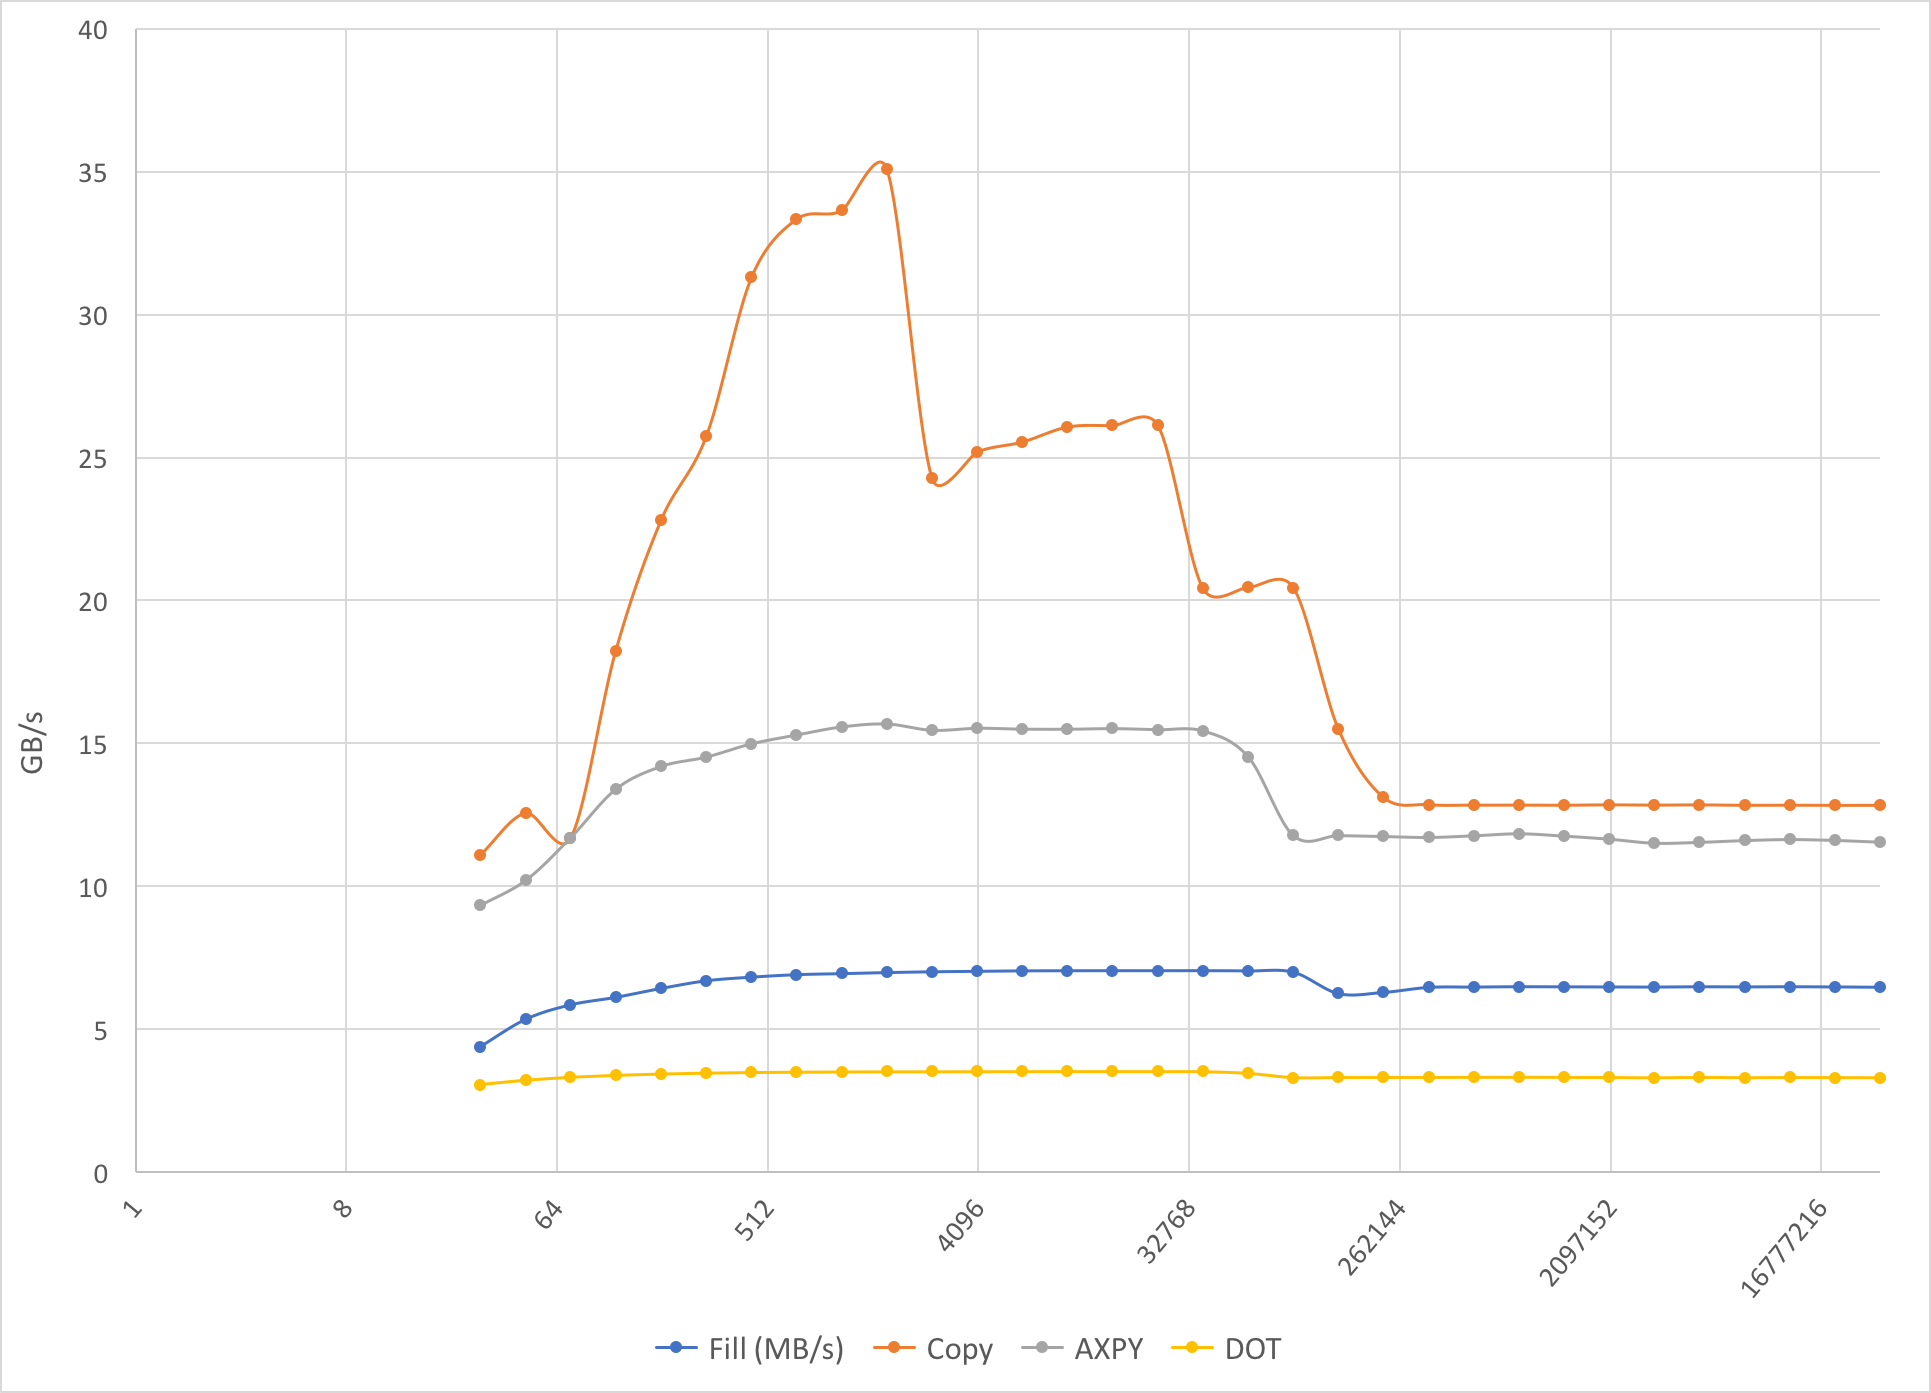
\includegraphics[width=15cm,keepaspectratio]{imgs/img01.png}
\end{figure} 

\newpage

The other measure to identify how far the nbody problem is from the ideal speed we compute the efficient. In Figure.2 we can see how as the threads increased depending of the particles sized the efficiency of the parallel program decreased. 

This is due to that in many cases starting the parallelize regions creates an overhead that when the problem size doesnt scale proportionally to the number of threads the program efficiency decreased significantly. 

\begin{figure}[htb]
\caption{Strong Scaling - Efficiency (Sp/P)}\label{fig:benchmark01}
\centering
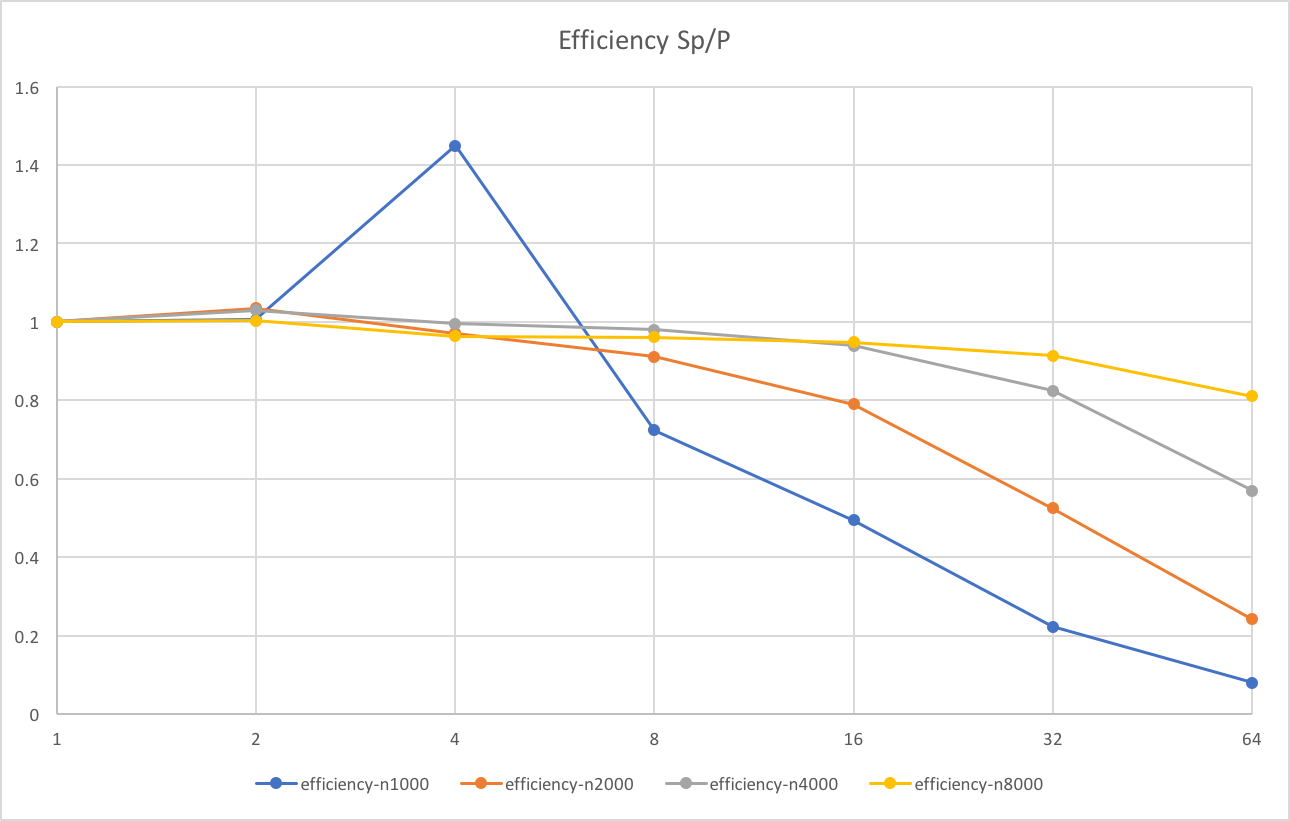
\includegraphics[width=\textwidth,keepaspectratio]{imgs/img02.png}
\end{figure} 

\newpage

\subsection{Weak scalability}

A more realistic accurate way to measure the speed-up, efficiency of a parallel program, would distribute the data amount all threads in order to avoid idling due to some threads having less data to process. To summarize when we use more than thread communications between threads increased which creates an overhead. Now when the data is not distributed evenly between threads then we would have some threads idling. These are some of the reason why the actual speedup and efficiency of the parallel program decreased. For the case of weak scalability on the nbody problem as the particles and threads increase we want to keep the amount of data per thread to stay constant or as close to constant as possible to achieve constant execution time. 

In Figure.3 we can see how there is a near perfect scalability as the threads and particles increased.

\begin{figure}[htb]
\caption{Weak Scaling - Speed-Up (T1/Tp)}\label{fig:benchmark02}
\centering
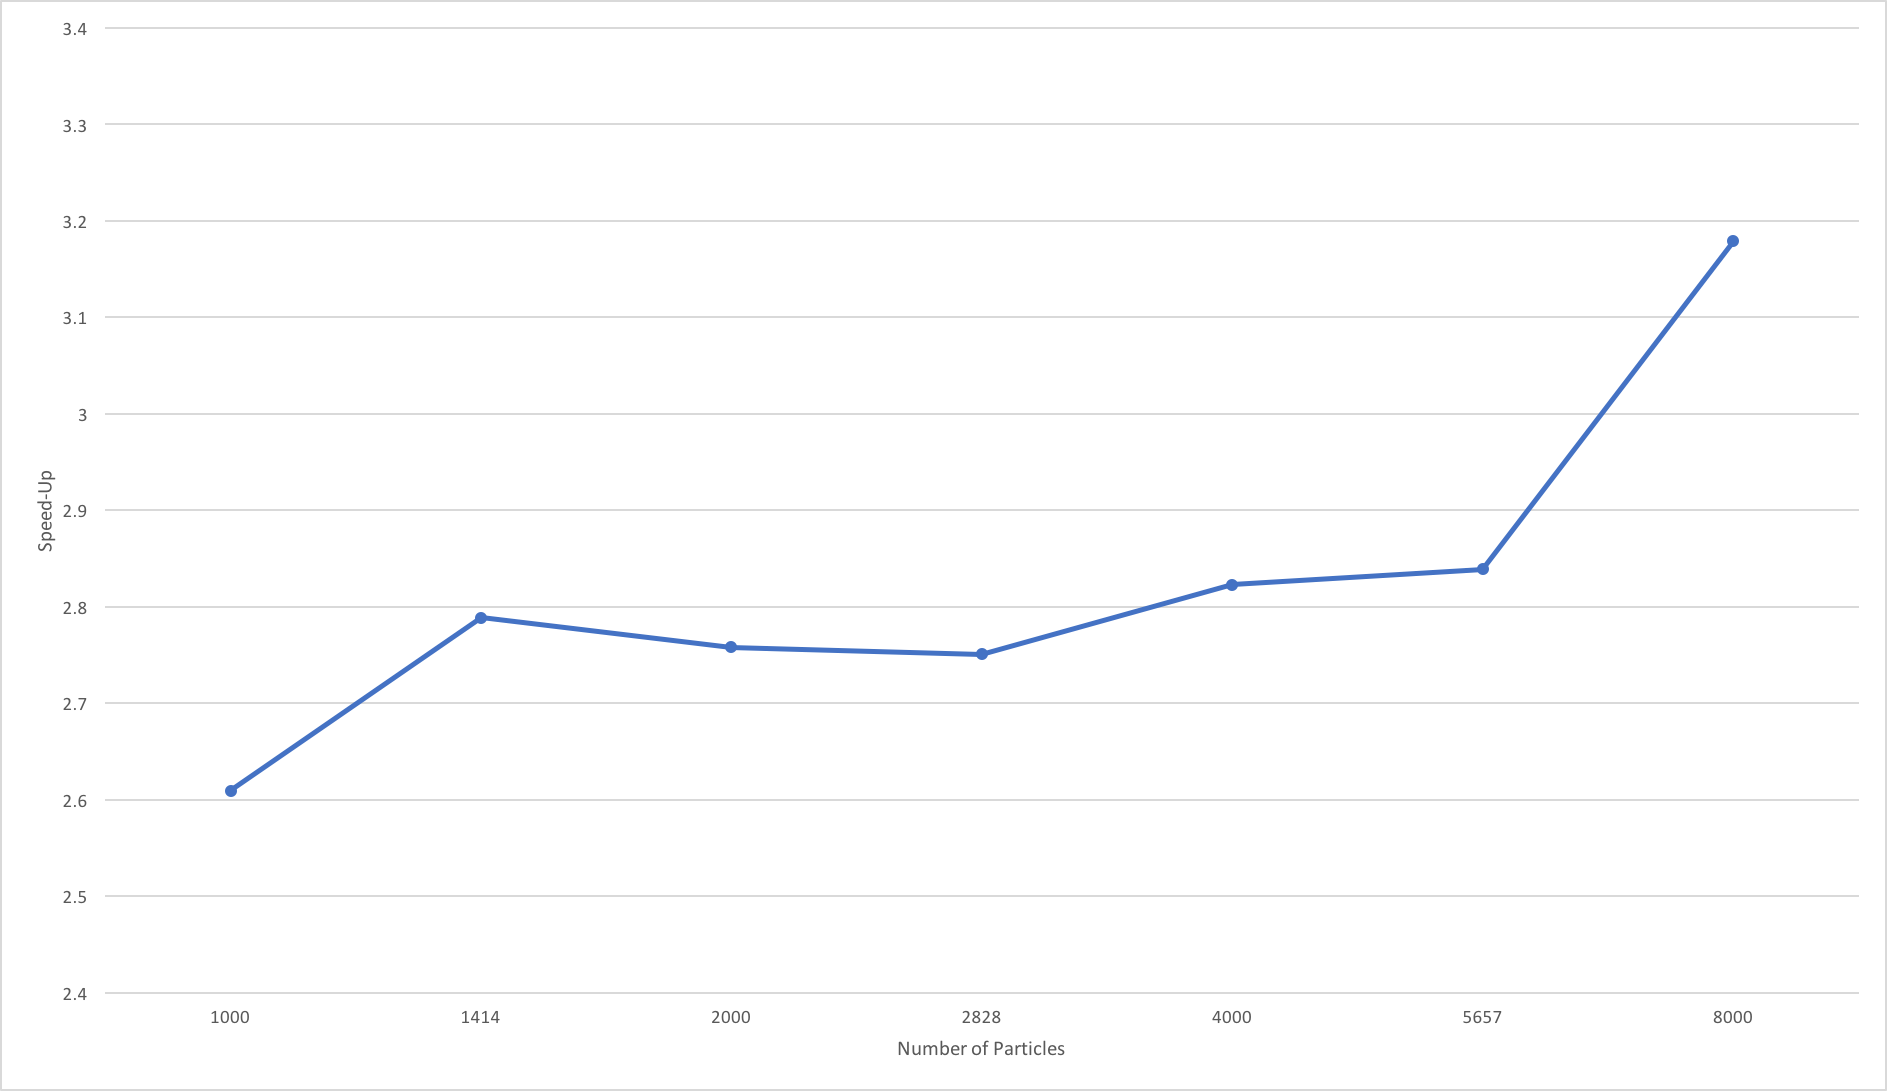
\includegraphics[width=\textwidth,keepaspectratio]{imgs/img03.png}
\end{figure}

\newpage

For the case of week scalability efficiency in Figure.4 the numbers of particles are given by the recursive function $ P_i = \sqrt{2} \times P_{i-1} $. We can see how for the first couple of threads efficiency is constant or close to constant as the amount of data that each thread process stays close to constant.

\begin{figure}[htb]
\caption{Weak Scaling - Efficiency (Sp/P)}\label{fig:benchmark02}
\centering
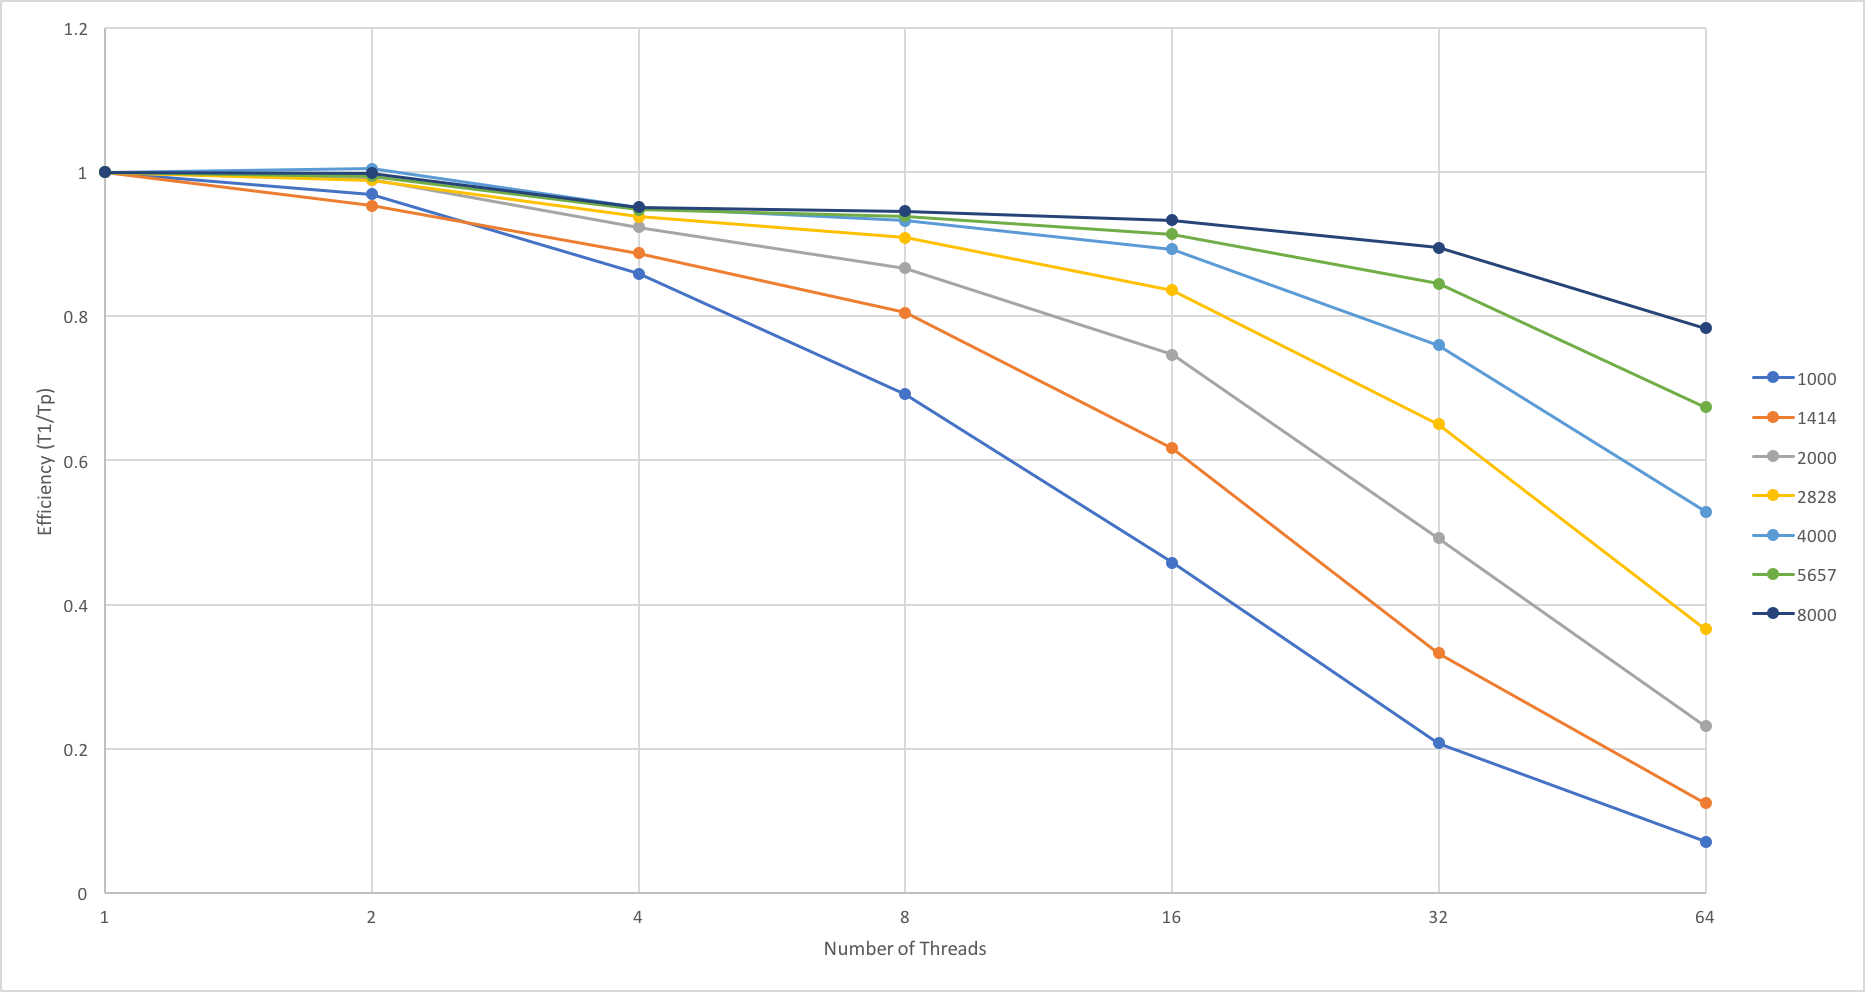
\includegraphics[width=\textwidth,keepaspectratio]{imgs/img04.png}
\end{figure}


%----------------------------------------------------------------
%	SECTION 3 - REFERENCE
%----------------------------------------------------------------

\section{Reference}

\begin{flushleft}
Stampede2 User Guide -- Managing Memory \\ \url{https://portal.tacc.utexas.edu/user-guides/stampede2#managingmemory}

Introduction to High Performance Scientific Computing -- Victor Eijkhout \\ \url{http://pages.tacc.utexas.edu/~eijkhout/istc/istc.html}
\end{flushleft}

\newpage


\begin{table}[]
\centering
\caption{Strong Scaling Benchmark - Number of Particles: 1000}
\resizebox{\textwidth}{!}{%
\begin{tabular}{@{}cccc@{}}
\toprule
\textbf{Threads} & \textbf{runtime-n1000} & \textbf{speed-up-n1000} & \textbf{efficiency-n1000} \\ \midrule
1 & 2.699547 & 1.00 & 1.00 \\
2 & 1.342266 & 2.01 & 1.01 \\
4 & 0.767273 & 3.52 & 0.88 \\
8 & 0.465877 & 5.79 & 0.72 \\
16 & 0.340848 & 7.92 & 0.50 \\
32 & 0.378338 & 7.14 & 0.22 \\
64 & 0.527209 & 5.12 & 0.08 \\ \bottomrule
\end{tabular}%
}
\end{table}

\begin{table}[]
\centering
\caption{Strong Scaling Benchmark - Number of Particles: 2000}
\resizebox{\textwidth}{!}{%
\begin{tabular}{@{}cccc@{}}
\toprule
\textbf{Threads} & \textbf{runtime-n2000} & \textbf{speed-up-n2000} & \textbf{efficiency-n2000} \\ \midrule
1 & 10.702174 & 1.00 & 1.00 \\
2 & 5.170901 & 2.07 & 1.03 \\
4 & 2.755932 & 3.88 & 0.97 \\
8 & 1.468389 & 7.29 & 0.91 \\
16 & 0.846486 & 12.64 & 0.79 \\
32 & 0.636906 & 16.80 & 0.53 \\
64 & 0.689989 & 15.51 & 0.24 \\ \bottomrule
\end{tabular}%
}
\end{table}

\begin{table}[]
\centering
\caption{Strong Scaling Benchmark - Number of Particles: 4000}
\resizebox{\textwidth}{!}{%
\begin{tabular}{@{}cccc@{}}
\toprule
\textbf{Threads} & \textbf{runtime-n4000} & \textbf{speed-up-n4000} & \textbf{efficiency-n4000} \\ \midrule
1 & 42.174895 & 1.00 & 1.00 \\
2 & 20.477445 & 2.06 & 1.03 \\
4 & 10.593958 & 3.98 & 1.00 \\
8 & 5.375854 & 7.85 & 0.98 \\
16 & 2.804787 & 15.04 & 0.94 \\
32 & 1.598818 & 26.38 & 0.82 \\
64 & 1.155382 & 36.50 & 0.57 \\ \bottomrule
\end{tabular}%
}
\end{table}

\begin{table}[]
\centering
\caption{Strong Scaling Benchmark - Number of Particles: 8000}
\resizebox{\textwidth}{!}{%
\begin{tabular}{@{}cccc@{}}
\toprule
\textbf{Threads} & \textbf{runtime-n8000} & \textbf{speed-up-n8000} & \textbf{efficiency-n8000} \\ \midrule
1 & 161.399121 & 1.00 & 1.00 \\
2 & 80.410162 & 2.01 & 1.00 \\
4 & 41.872722 & 3.85 & 0.96 \\
8 & 21.005236 & 7.68 & 0.96 \\
16 & 10.634796 & 15.18 & 0.95 \\
32 & 5.517657 & 29.25 & 0.91 \\
64 & 3.109065 & 51.91 & 0.81 \\ \bottomrule
\end{tabular}%
}
\end{table}

\begin{table}[]
\centering
\caption{Weak Scaling Benchmark - Number of Particles: 1000}
\resizebox{\textwidth}{!}{%
\begin{tabular}{@{}cccc@{}}
\toprule
\textbf{Threads} & \textbf{runtime-n1000} & \textbf{speed-up-n1000} & \textbf{efficiency-n1000} \\ \midrule
1 & 2.609648 & 1.00 & 1.00 \\
2 & 1.346056 & 1.94 & 0.97 \\
4 & 0.759546 & 3.44 & 0.86 \\
8 & 0.471636 & 5.53 & 0.69 \\
16 & 0.356043 & 7.33 & 0.46 \\
32 & 0.393292 & 6.64 & 0.21 \\
64 & 0.57277 & 4.56 & 0.07 \\ \bottomrule
\end{tabular}%
}
\end{table}

\begin{table}[]
\centering
\caption{Weak Scaling Benchmark - Number of Particles: 1414}
\resizebox{\textwidth}{!}{%
\begin{tabular}{@{}cccc@{}}
\toprule
\textbf{Threads} & \textbf{runtime-n1414} & \textbf{speed-up-n1414} & \textbf{efficiency-n1414} \\ \midrule
1 & 5.316273 & 1.00 & 1.00 \\
2 & 2.788752 & 1.91 & 0.95 \\
4 & 1.497149 & 3.55 & 0.89 \\
8 & 0.825781 & 6.44 & 0.80 \\
16 & 0.538592 & 9.87 & 0.62 \\
32 & 0.499729 & 10.64 & 0.33 \\
64 & 0.667798 & 7.96 & 0.12 \\ \bottomrule
\end{tabular}%
}
\end{table}

\begin{table}[]
\centering
\caption{Weak Scaling Benchmark - Number of Particles: 2000}
\resizebox{\textwidth}{!}{%
\begin{tabular}{@{}cccc@{}}
\toprule
\textbf{Threads} & \textbf{runtime-n2000} & \textbf{speed-up-n2000} & \textbf{efficiency-n2000} \\ \midrule
1 & 10.186014 & 1.00 & 1.00 \\
2 & 5.148521 & 1.98 & 0.99 \\
4 & 2.757893 & 3.69 & 0.92 \\
8 & 1.468954 & 6.93 & 0.87 \\
16 & 0.852953 & 11.94 & 0.75 \\
32 & 0.647286 & 15.74 & 0.49 \\
64 & 0.688234 & 14.80 & 0.23 \\ \bottomrule
\end{tabular}%
}
\end{table}

\begin{table}[]
\centering
\caption{Weak Scaling Benchmark - Number of Particles: 2828}
\resizebox{\textwidth}{!}{%
\begin{tabular}{@{}cccc@{}}
\toprule
\textbf{Threads} & \textbf{runtime-n2828} & \textbf{speed-up-n2828} & \textbf{efficiency-n2828} \\ \midrule
1 & 20.007112 & 1.00 & 1.00 \\
2 & 10.115954 & 1.98 & 0.99 \\
4 & 5.331802 & 3.75 & 0.94 \\
8 & 2.751072 & 7.27 & 0.91 \\
16 & 1.495437 & 13.38 & 0.84 \\
32 & 0.960981 & 20.82 & 0.65 \\
64 & 0.854334 & 23.42 & 0.37 \\ \bottomrule
\end{tabular}%
}
\end{table}

\begin{table}[]
\centering
\caption{Weak Scaling Benchmark - Number of Particles: 4000}
\resizebox{\textwidth}{!}{%
\begin{tabular}{@{}cccc@{}}
\toprule
\textbf{Threads} & \textbf{runtime-n4000} & \textbf{speed-up-n4000} & \textbf{efficiency-n4000} \\ \midrule
1 & 40.344163 & 1.00 & 1.00 \\
2 & 20.077003 & 2.01 & 1.00 \\
4 & 10.612086 & 3.80 & 0.95 \\
8 & 5.409125 & 7.46 & 0.93 \\
16 & 2.822763 & 14.29 & 0.89 \\
32 & 1.659283 & 24.31 & 0.76 \\
64 & 1.192224 & 33.84 & 0.53 \\ \bottomrule
\end{tabular}%
}
\end{table}

\begin{table}[]
\centering
\caption{Weak Scaling Benchmark - Number of Particles: 5657}
\resizebox{\textwidth}{!}{%
\begin{tabular}{@{}cccc@{}}
\toprule
\textbf{Threads} & \textbf{runtime-n5657} & \textbf{speed-up-n5657} & \textbf{efficiency-n5657} \\ \midrule
1 & 76.810418 & 1.00 & 1.00 \\
2 & 38.630002 & 1.99 & 0.99 \\
4 & 20.254395 & 3.79 & 0.95 \\
8 & 10.229366 & 7.51 & 0.94 \\
16 & 5.252118 & 14.62 & 0.91 \\
32 & 2.839027 & 27.06 & 0.85 \\
64 & 1.781306 & 43.12 & 0.67 \\ \bottomrule
\end{tabular}%
}
\end{table}

\begin{table}[]
\centering
\caption{Weak Scaling Benchmark - Number of Particles: 8000}
\resizebox{\textwidth}{!}{%
\begin{tabular}{@{}cccc@{}}
\toprule
\textbf{Threads} & \textbf{runtime-n8000} & \textbf{speed-up-n8000} & \textbf{efficiency-n8000} \\ \midrule
1 & 159.344296 & 1.00 & 1.00 \\
2 & 79.801012 & 2.00 & 1.00 \\
4 & 41.869284 & 3.81 & 0.95 \\
8 & 21.055475 & 7.57 & 0.95 \\
16 & 10.666953 & 14.94 & 0.93 \\
32 & 5.562885 & 28.64 & 0.90 \\
64 & 3.178754 & 50.13 & 0.78 \\ \bottomrule
\end{tabular}%
}
\end{table}


\begin{figure}[]
\caption{OpenMP Pragmas for Acceleration Function}\label{fig:benchmark01}
\begin{lstlisting}
template <typename ValueType>
void accel_register (	ValueType * __RESTRICT pos, 
			ValueType * __RESTRICT vel, 
			ValueType * __RESTRICT mass, 
			ValueType * __RESTRICT acc, 
			const int n)
{
   #pragma omp parallel
    {
    #pragma omp for
       for (int i = 0; i < n; ++i)
       {
          ValueType ax = 0, ay = 0, az = 0;
          const ValueType xi = pos_array(i,0);
          const ValueType yi = pos_array(i,1);
          const ValueType zi = pos_array(i,2);
          for (int j = 0; j < n; ++j)
          {
             /* Position vector from i to j and the distance^2. */
             ValueType rx = pos_array(j,0) - xi;
             ValueType ry = pos_array(j,1) - yi;
             ValueType rz = pos_array(j,2) - zi;
             ValueType dsq = rx*rx + ry*ry + rz*rz + TINY2;
             ValueType m_invR3 = mass[j] / (dsq * std::sqrt(dsq));
    
             ax += rx * m_invR3;
             ay += ry * m_invR3;
             az += rz * m_invR3;
          }
    
          acc_array(i,0) = G * ax;
          acc_array(i,1) = G * ay;
          acc_array(i,2) = G * az;
       }
    }
}
\end{lstlisting}
\end{figure}

\begin{figure}[]
\caption{OpenMP Pragmas for Update Function}\label{fig:benchmark01}
\begin{lstlisting}
template <typename ValueType>
void update (ValueType pos[], ValueType vel[], ValueType mass[], ValueType acc[], const int n, ValueType h)
{
    #pragma omp parallel
    {
    #pragma omp for
       for (int i = 0; i < n; ++i)
          for (int k = 0; k < NDIM; ++k)
          {
             pos_array(i,k) += vel_array(i,k)*h + acc_array(i,k)*h*h/2;
             vel_array(i,k) += acc_array(i,k)*h;
          }
    }
}
\end{lstlisting}
\end{figure}

\begin{figure}[]
\caption{OpenMP Pragmas for Search Function}\label{fig:benchmark01}
\begin{lstlisting}
template <typename ValueType>
void search (ValueType pos[], ValueType vel[], ValueType mass[], ValueType acc[], const int n)
{
  ValueType minv = 1e10, maxv = 0, ave = 0;
  #pragma omp parallel default(none) shared(minv,maxv,ave)
  {
  #pragma omp for reduction(+:ave) reduction(max:maxc) reduction(min:minv)       
   for (int i = 0; i < n; ++i)
   {
         ValueType vmag = 0;
         for (int k = 0; k < NDIM; ++k)
         	vmag += (vel_array(i,k) * vel_array(i,k));
         vmag = sqrt(vmag);
         maxv = std::max(maxv, vmag);
         minv = std::min(minv, vmag);
         ave += vmag;
    }
   printf("min/max/ave velocity = %e, %e, %e\n", minv, maxv, ave/n);
  }
}
\end{lstlisting}
\end{figure}

\begin{table}[]
\centering
\caption{Stampede2 - Compute Node (knl) - System Information}
\resizebox{\textwidth}{!}{%
\begin{tabular}{@{}ll@{}}
\toprule
\textbf{Architecture} & x86\_64 \\ \midrule
\textbf{CPU op-mode(s)} & 32-bit, 64-bit \\
\textbf{Byte Order} & Little Endian \\
\textbf{CPU(s)} & 272 \\
\textbf{On-line CPU(s) list} & 0-271 \\
\textbf{Thread(s) per core} & 4 \\
\textbf{Core(s) per socket} & 68 \\
\textbf{Socket(s)} & 1 \\
\textbf{NUMA node(s)} & 2 \\
\textbf{Vendor ID} & GenuineIntel \\
\textbf{CPU family} & 6 \\
\textbf{Model} & 87 \\
\textbf{Model name} & Intel(R) Xeon Phi(TM) CPU 7250 @ 1.40GHz \\
\textbf{Stepping} & 1 \\
\textbf{CPU MHz} & 1255.132 \\
\textbf{BogoMIPS} & 2793.44 \\
\textbf{L1d cache} & 32K \\
\textbf{L1i cache} & 32K \\
\textbf{L2 cache} & 1024K \\
\textbf{NUMA node0 CPU(s)} & 0-271 \\
\textbf{NUMA node1 CPU(s)} &  \\ \bottomrule
\end{tabular}%
}
\end{table}


\end{document}